% !TeX root = ../paper.tex

\section{Optimal Transport for Dimension Reduction with SNEkhorn}\label{sec:DR_with_OT}

In this section, we build upon symmetric entropic affinities to introduce SNEkhorn, a new DR algorithm that fully benefits from the advantages of doubly stochastic affinities.

\paragraph{SNEkhorn's objective.} Our proposed method relies on doubly stochastic affinity matrices to capture the dependencies among the samples in both input \emph{and} latent spaces. The $\KL$ divergence, which is the central criterion in most popular DR methods \cite{van2022probabilistic}, is used to measure the discrepancy between the two affinities. As detailed in sections \ref{sec:background} and \ref{sec:sym_entropic_affinity}, $\Pb^{\mathrm{se}}$ corrects for heterogeneity in the
data density by imposing point-wise entropy constraints. As we do not need such correction for embedding coordinates $\Z$ since they must be optimized, we opt for the standard affinity \eqref{eq:plan_sym_sinkhorn} built as an OT transport plan with global entropy constraint \eqref{eq:entropy_constrained_OT}. This OT plan can be efficiently computed using Sinkhorn's algorithm. More precisely, 
% considering $\C_\X$ and $\C_{\Zb}$  the pairwise cost matrices of $\X$ and $\Z$ respectively, 
we propose the optimization problem
\begin{align}\label{coupling_pb}
    \min_{\Zb \in \mathbb{R}^{n \times q}} \:  \mathrm{KL}\big(\Pb^{\mathrm{se}} | \mathbf{Q}^{\mathrm{ds}}_{\Zb} \big)\,,
\tag{SNEkhorn}
\end{align}
where $\mathbf{Q}^{\mathrm{ds}}_{\Zb} = \exp \left(\mathbf{f}_{\Zb} \oplus \mathbf{f}_{\Zb} - \C_{\Zb} \right)$ stands for the $\eqref{eq:plan_sym_sinkhorn}$ affinity computed with cost $\C_{\Zb}$ and $\mathbf{f}_{\Zb}$ is the optimal dual variable found by Sinkhorn's algorithm.
% In the above, $\Pb^{\mathrm{se}}_{\xi}(\C_\X)$ stands for the \eqref{eq:sym_entropic_affinity} matrix associated to the cost $\C_\X$ with perplexity $\xi$. 
We set the bandwidth to $\nu = 1$ in $\Qb^{\mathrm{ds}}_{\Zb}$ similarly to \cite{van2008visualizing} as the bandwidth in the low dimensional space only affects the scales of the embeddings and not their shape.
Keeping only the terms that depend on $\Z$ and relying on the double stochasticity of $\Pb^{\mathrm{se}}$, the objective in (\ref{coupling_pb}) can be expressed as $\langle \Pb^{\mathrm{se}}, \C_{\Zb} \rangle - 2 \langle \mathbf{f}_{\Zb}, \bm{1} \rangle$. %In this decomposition, the left term settles attractive forces and the right term repulsive ones. pas tres clair j'enelve

\textbf{Heavy-tailed kernel in latent space.}
Since it is well known that heavy-tailed kernels can be beneficial in DR
\cite{kobak2020heavy}, we propose an extension called t-SNEkhorn that
simply amounts to computing a doubly stochastic student-t kernel 
% $\Tilde{\K} = (\bm{1}\bm{1}^\top + \C)^{\odot -1}$ 
in the low-dimensional space. With our construction, it corresponds to choosing the cost $[\C_{\Zb}]_{ij} = \left(\log(1 + \|\Z_{i:}-\Z_{j:}\|_2^2)\right)_{ij}$
instead of $(\|\Z_{i:}-\Z_{j:}\|_2^2)_{ij}$.

\textbf{Inference.}
This new DR objective involves computing a doubly stochastic normalization for each update of $\Z$. Interestingly, to compute the optimal dual variable $\mathbf{f}_{\Zb}$ in $\Qb^{\mathrm{ds}}_{\Zb}$, we leverage a well-conditioned Sinkhorn fixed point iteration \citep{knight2014symmetry, feydy2019interpolating}, which converges extremely fast in the symmetric setting:
\begin{equation}\label{eq:sinkhorn_iterations_log_sym_accelerated}
    \forall i, \: 
    [\mathbf{f}_{\Zb}]_i \leftarrow \frac{1}{2} \left( [\mathbf{f}_{\Zb}]_i - \log \sum_{k} \exp \big([\mathbf{f}_{\Zb}]_k - [\Cb_{\Zb}]_{ki} \big) \right) \:.
\tag{Sinkhorn}
\end{equation}
On the right side of \cref{fig:snekhorn_not_DS}, we plot $\| \Qb^{\mathrm{ds}}_{\Zb} \bm{1} - \bm{1} \|_{\infty}$ as a function of \eqref{eq:sinkhorn_iterations_log_sym_accelerated} iterations for a toy example presented in \cref{sec:DR_experiments}. In most practical cases, we found that about 10 iterations were enough to reach sufficiently small error. 
$\Z$ is updated through gradient descent with gradients obtained by performing
backpropagation through the Sinkhorn iterations. These
iterations can be further accelerated with a \emph{warm start} strategy by plugging the $\mathbf{f}_{\Zb}$ of the
last Sinkhorn to initialize the current one.
% Fortunately, one doesn't need to differentiate through all the unrolled Sinkhorn iterations (\ref{eq:sinkhorn_iterations_log_sym_accelerated}) to compute $\nabla_{\Zb}\f$.
% One can derive the gradient of the objective \textit{w.r.t.}\ $\Z$ as
% \begin{align*}
%     \nabla_{\Zb} \mathcal{J}(\X, \Z) = 2 \left(\Lb \Z - \nabla_{\Zb}\f^{\top} \bm{1} \right) \:.
% \end{align*} 

\begin{minipage}{0.59\linewidth}
        \textbf{Related work.}
        Using doubly stochastic affinities for SNE has been proposed in \cite{lu2019doubly}, with two key differences from our work. First, they
        do not consider EAs and resort to $\Pb^{\mathrm{ds}}$ \eqref{eq:plan_sym_sinkhorn}. This affinity, unlike $\Pb^{\mathrm{se}}$, is not adaptive to the data heterogeneous density (as illusrated in \cref{fig:Ps_vs_Pse}). 
        Second, they use the affinity $\widetilde{\Qb}_{\Zb}$ in the low-dimensional space and demonstrate both empirically and theoretically that matching the latter with a doubly stochastic matrix (\eg $\Pb^{\mathrm{ds}}$ or $\Pb^{\mathrm{se}}$) imposes spherical constraints on the embedding $\Z$.
        % As a consequence, latent coordinates tend to concentrate on spheres \titouan{pas clair: DS + pas DS = sphere, DS + DS = pas sphere ?}. As a consequence, they focus on building embeddings on spheres in a $3D$ space.
        This is detrimental for projections onto a $2D$ flat space (typical use case of DR) where embeddings tend to form circles. This can be verified on the left side of \cref{fig:snekhorn_not_DS}. In contrast, in SNEkhorn, the latent affinity \emph{is also doubly stochastic} so that latent coordinates $\Z$ are not subject to spherical constraints anymore.
        The corresponding SNEkhorn embedding is shown in \cref{fig:simulated_data_multinomial} (bottom right).
        % their proposed method called \texttt{DOSNES} does
\end{minipage}
\hspace{0.005\linewidth}
\begin{minipage}{0.4\linewidth} 
\vspace{-0.2cm}
    \centerline{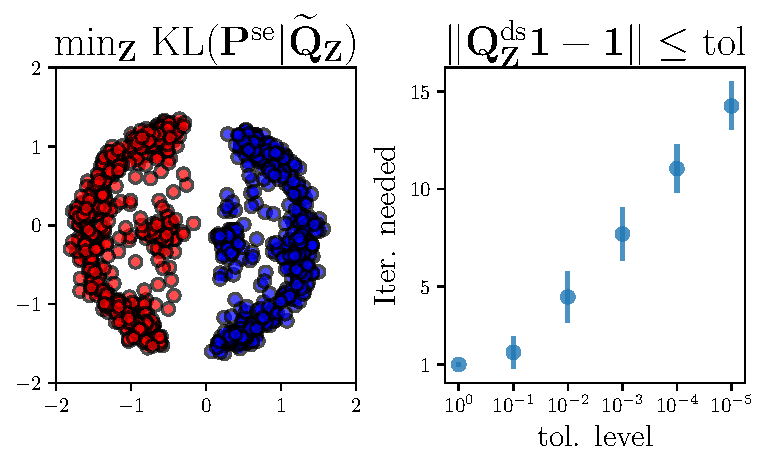
\includegraphics[width=\linewidth]{figures/snekhorn_not_DS.pdf}}
    \captionof{figure}{Left: SNEkhorn embedding on the simulated data of \cref{sec:DR_experiments} using $\widetilde{\Qb}_{\Zb}$ instead of $\Qb^{\mathrm{ds}}_{\Zb}$ with $\xi=30$. Right: number of iterations needed to achieve $\| \Qb^{\mathrm{ds}}_{\Zb} \bm{1} - \bm{1} \|_{\infty} \leq \text{tol}$ with \eqref{eq:sinkhorn_iterations_log_sym_accelerated}.}
    \label{fig:snekhorn_not_DS}
\end{minipage}
